\documentclass[dvipsnames, svgnames, x11names, a4paper, 11pt]{article}

% URLs and hyperlinks ------------------------------
\usepackage{hyperref}
\hypersetup{
    colorlinks=true,
    linkcolor=NavyBlue,
    filecolor=magenta,      
    urlcolor=blue,
}
\usepackage{xurl}
%---------------------------------------------------

\usepackage{float}
\usepackage{graphicx}
\usepackage{listings}
\usepackage{color}
\usepackage{xcolor}
\usepackage{subfigure}

\definecolor{dkgreen}{rgb}{0,0.6,0}
\definecolor{gray}{rgb}{0.5,0.5,0.5}
\definecolor{mauve}{rgb}{0.58,0,0.82}

\lstset{frame=tb,
    language=vhdl,
    aboveskip=3mm,
    belowskip=3mm,
    showstringspaces=false,
    columns=flexible,
    basicstyle=\ttfamily,
    numbers=left,
    numberstyle=\small\color{gray},
    keywordstyle=\bfseries\color{Green4},
    commentstyle=\color{gray},
    stringstyle=\color{mauve},
    breaklines=true,
    breakatwhitespace=true,
    tabsize=4,
    identifierstyle=\color{black}
}

\usepackage{xepersian}
\settextfont{Yas}

\renewcommand{\abstractname}{توضیحات سایت\LTRfootnote{\url{https://posedge.ir/1399/07/21/connect-7segment-to-fpga/}}:
}
\title{تمرین \lr{7-Segement}}
\author{
فاطمه علی‌ملکی \\
مهدی حق‌وردی
}

\begin{document}
\maketitle
\tableofcontents

\section{اتصال چهار \lr{7-Segment} به برد \lr{FPGA}}
\begin{abstract}
آیا ما از 4 عدد \lr{7-Segment} استفاده کنیم و هر \lr{7-Segment}، ۹ پایه احتیاج داشته باشد باید برای نمایش مقدار مورد نظر از 36 پایه fpga استفاده کنیم؟ \\

خیر این‌گونه نیست. باید گفت که پایه های
\lr{enable}
هر کدام به یک پورت متصل شود ولی بر فرض مثال پایه \lr{a} هر چهار \lr{7-Segment} باید تنها به یک پورت متصل شود.

باید به این نکته توجه کرد که چشم انسان توانایی دیدن روشن خاموش شدن مداوم یک \lr{LED} را تا فرکانس (سرعت) مشخصی دارد و اگر سرعت خاموش و روشن شدن آن بر فرض مثال به 8 میلی ثانیه برسد چشم انسان  قادر به تشخیص دقیق آن نخواهد بود .

حال فرض کنیم عبارت 2020 قرار است توسط 4 عدد \lr{7-Segment} نمایش داده شود ابتدا در لحظه صفر پایه \lr{enable} اولی وصل میشود  و بقیه \lr{enable} ها قطع میشوند و پورت های 
\lr{a}،
\lr{b}،
\lr{c}،
\lr{d}، 
\lr{e}،
\lr{f} و
\lr{g}
مقدار صفر را نمایش میدهند و بعد از 8 میلی ثانیه (دلخواه) \lr{enable} دوم فعال و بقیه غیر فعال میشوند و پورتها مقدار دو را نمایش میدهند ، اگر همینگونه این کار ادامه یابد و تکرار شود چشم ما تنها مقادیر 2020 را خواهد دید تنها با تعداد پورت مصرفی کمتر.
\end{abstract}\label{abstract}
''به طور خلاصه در یک لحظه تنها یکی از \lr{7-Segment}ها، روشن است اما چون تعویض به سرعت اتفاق میوفتد، چشم ما توانایی دیدن روشن و خاموش شدن آنها را ندارد.``

\section{توضیح فایل‌های \lr{VHDL}}
\subsection{فایل \lr{\texttt{clock\_divide.vhd}}}\label{sec:cd}
\subsection{فایل \lr{\texttt{decodeSevenSeg.vhd}}}\label{sec:dss}
\subsection{فایل \lr{\texttt{sevenSegment.vhd}}}\label{sec:ss}

\section{چالش‌ها}
در این قسمت به توضیح چالش‌های مطرح شده، می‌پردازیم.

\subsection{چالش اول}
طبق توضیحاتی که در 
(\ref{abstract})
آمد، ما باید در فایل 
\lr{\texttt{clock\_divide.vhd}}
تغییراتی را اعمال کنیم که تعداد بار روشن شدن هر یک از 
\lr{7-Segment}ها
آنقدری زیاد بشود، که چشم انسان قابلیت تشخیص روشن خاموش شدن آنها را نداشته باشد.
\textbf{این یعنی عدد‌هایی که در این فایل‌ هستند باید کوچک‌تر شوند تا سرعت خاموش روشن شدن افزایش یابد.}
چون در زمان نوشتن این گزارش هنوز آزمایش را انجام نداده‌ایم عدد دقیق آن را نمیدانیم\RTLfootnote{در زمان آزمایش عدد آنها را روی فایل گزارش با خودکار می‌شود.} اما مکان‌ کد‌هایی که باید تغییر کنند در تصویر
\ref{fig:cd}
آمده‌اند.\RTLfootnote{پرانتز‌ها}
\subsection{چالش سوم}

\begin{figure}[b]
\begin{center}
\subfigure
[تغییرات کلاک]
{\label{fig:cd}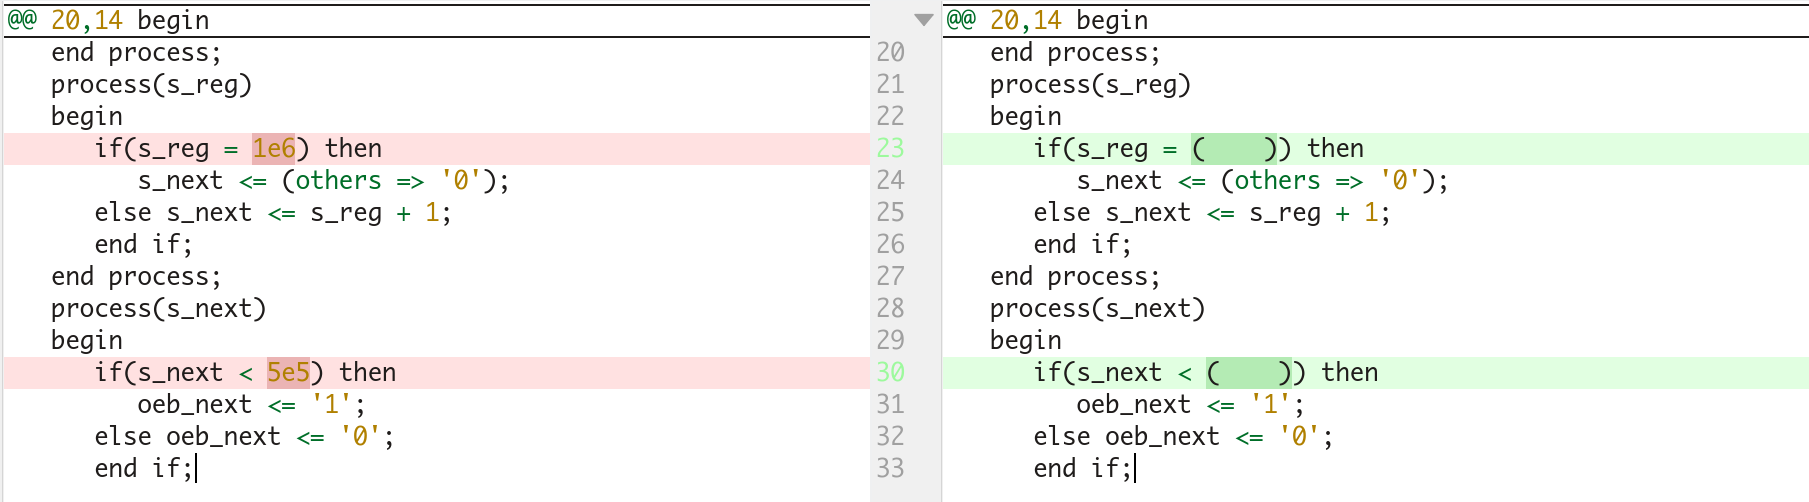
\includegraphics[width=0.90\textheight, height=0.43\textwidth, angle=90]{./images/cd}
}
\end{center}
\end{figure}
\listoffigures
\end{document}